\chapter{Physical aspects of Fluid-Structure Interaction problems}
\label{cha:physics}


Dynamic models of solids or fluids aim at describing the evolution of an initial configuration through time. Structural mechanics and fluid dynamics use different perspectives when describing the motion of respectively a solid or a fluid particle. When dealing with FSI problems the two approaches need to be combined in order to obtain a suitable description of the two domains and their interface: this aspect is treated in \ref{sec:desc-motion}.

As outlined in the introduction, the fluid and the solid domain of a FSI problem might be described by means of many different models: some of them are outlined in section \ref{sec:models}.  \textit{Dimensional analysis} and the use of dimensionless numbers is a powerful tool used to classify fluid dynamics problems: some of the principles used there can be applied to FSI problems in order to classify them: this can help define and classify FSI problems, as described in section \ref{sec:classification}.

\section{Description of motion}
\label{sec:desc-motion}

In a FSI model, the fluid in motion deforms the solid because of the forces exerted to the structure. The change in the shape of the solid modifies the fluid domain, causing a different flow behavior. For this reason it is necessary to describe formally the kinematics and the dynamics of the whole process. Classical continuum mechanics considers the motion of particles by means of two different perspectives  \cite{batra2006elements}: the \textit{Eulerian description}, briefly described in section \ref{subsec:euler}, and the \textit{Lagrangian description}, outlined in section \ref{subsec:lagrange}. Those two perspectives are typically combined into the \textit{~\ac{ALE}} method, described in section \ref{subsec:ALE}.

\subsection{Eulerian perspective}
\label{subsec:euler}

The \textit{Eulerian perspective} observes the change of quantities of interest (e.g. density, velocity, pressure) at spatially fixed locations. In other words: the observer does not vary the point of view during different time steps. Thus, quantities can be expressed as functions of time at fixed locations. 
This is represented by the following notation:

\begin{equation}
	\Theta = \tilde{\Theta}(x,y,z,t)
	\label{eq:eulerian}
\end{equation}

where $\Theta$ is a quantity of interest and $\tilde{\Theta}$ denotes the same quantity form an Eulerian point of view; $(x, y, z)$ represent a fixed location in the euclidean space.


\begin{figure}[htbp!]
	\centering
	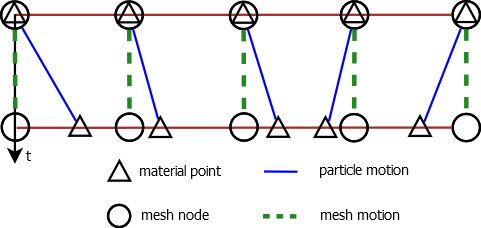
\includegraphics[width=0.8\textwidth]{images/eulerian}
	\caption{Eulerian perspective}
	\label{fig:eulerian}
\end{figure}

A computational mesh can be interpreted as a number of observers distributed across the domain of interest and connected to each other in order to form a a grid with nodes. If the particles of the domain move, a purely euclidean mesh does not move and the position other nodes remain fixed at any instance of time \cite{Cheng2006SlidingFL}. 
This behavior is represented in Figure \ref{fig:eulerian} (adapted from \cite{Cheng2006SlidingFL}). The mesh is independent of particles movement, resulting in a convenient choice for ~\ac{CFD} problems, where fluid flows throughout the whole
computational domain. Within this approach, proper mesh refinement is crucial for computational accuracy as it defines to what extent small scale movement can be modeled and resolved \cite{donea2017arbitrary}.

\subsection{Lagrangian perspective}
\label{subsec:lagrange}

A \textit{lagrangian observer} focuses on a single particles and follows it throughout the motion, as depicted in Figure \ref{fig:lagrangian}. Changes in the quantities of interest are observed at different spatial locations. 

\begin{figure}[htbp!]
	\centering
	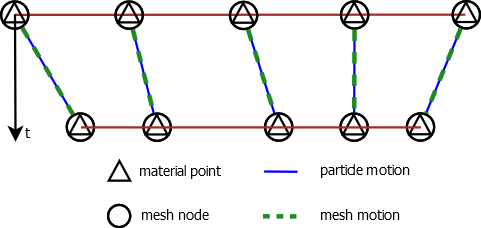
\includegraphics[width=0.8\textwidth]{images/lagrangian}
	\caption{Lagrangian perspective}
	\label{fig:lagrangian}
\end{figure}

The motion of the particle and the other quantities of interest can be described by reference coordinates (or \textit{material coordinates}) in Euclidean space $(X, Y, Z)$, uniquely identifying the observed particle at a reference configuration \cite{XING201957}. Usually $t = 0$ is chosen as reference but this is not mandatory. The Lagrangian observer only registers changes concerning one specific particle as time advances. Thus, quantities of interest can be described as:

\begin{equation}
	\Theta = \hat{\Theta}(X, Y, Z, t)
\end{equation}

In contrast to the Eulerian perspective (Equation \ref{eq:eulerian}), the obtained information is strictly limited to a single material particle (implied by the usage of the capital reference coordinate variables). 
Information about a fixed point in space is not directly available and no convective fluxes appear in a Lagrangian description.

This perspective is again translated into computational meshes: at a reference instance of time, mesh nodes are attached to material particles. As these move, the mesh nodes move with them causing the mesh to deform. Figure \ref{fig:lagrangian} describes the situation. The mesh nodes always coincide with their respective particles.

In this situation large-scale and irregular motions and more importantly deformation lead to distortions of the computational mesh, which yields smaller accuracy in simulations requiring to apply techniques to keep the desired accuracy \cite{lipton2010robustness}.

Lagrangian perspective is the usual method of choice for ~\ac{CSM} simulations.

Eulerian and Lagrangian descriptions are related \cite{bertram2012elasticity}. A mapping between them can described by the \textit{motion} function $\phi$ such that:


\begin{equation}
\vec{x}(t) = \phi(\vec{X}, t)
\label{eq:lag-motion}
\end{equation}

Equation \ref{eq:lag-motion} tells that he Eulerian, spatial position $\vec{x}$ of a particle at time t is the
mapping of the particle at its reference configuration $\vec{X}$: the mapping must be bijective.

\subsection{ALE method}
\label{subsec:ALE}

As outlined above, CSM and CFD problems adopt different perspectives. The ~\ac{ALE} approach, a combination of the two points of view, is used for FSI problems. As the name implies, an ALE observer moves arbitrarily with respect to a specific material particle.
Figure \ref{fig:ale} depicts such a situation.

\begin{figure}[htbp!]
	\centering
	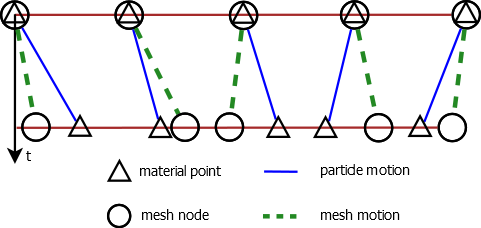
\includegraphics[width=0.8\textwidth]{images/ale}
	\caption{ALE perspective}
	\label{fig:ale}
\end{figure}

When dealing with computational meshes, an ALE mesh is considered as it can move almost arbitrarily with respect to the motion of the underlying particles, as shown in Figure \ref{fig:ale-mesh}.
The only constraint is that node movements should not distort the mesh too much as this leads to computational inaccuracy. Many algorithm exist to implement suitable quality criteria and keep the mesh motion reasonable and to allow the nodes to follow moving particles up to a certain extent \cite{de2007mesh}.

Since the mesh motion and material particle motion are not directly linked, a new unknown is introduced:  the relative movement between the ALE mesh and the material domain. This approach is particularly useful in FSI problems: fluid and solid must follow the moving interface between them for physical reasons.
Since the solid domain is usually described in a Lagrangian perspective, the solid mesh is kept attached to the FSI interface. However, also the fluid domain must deform to avoid formation of gaps between the meshes. Therefore, in ALE methods the fluid mesh nodes at the interface move with it. Fluid mesh nodes follow the fluid particles sticking to the interface (for viscous flows), while the rest of the fluid mesh is allowed to move in such way that mesh distortions are kept minimal, to preserve computational accuracy \cite{ramm1998fluid}.

\begin{figure}[htbp!]
	\centering
	\begin{subfigure}{.5\textwidth}
		\centering
		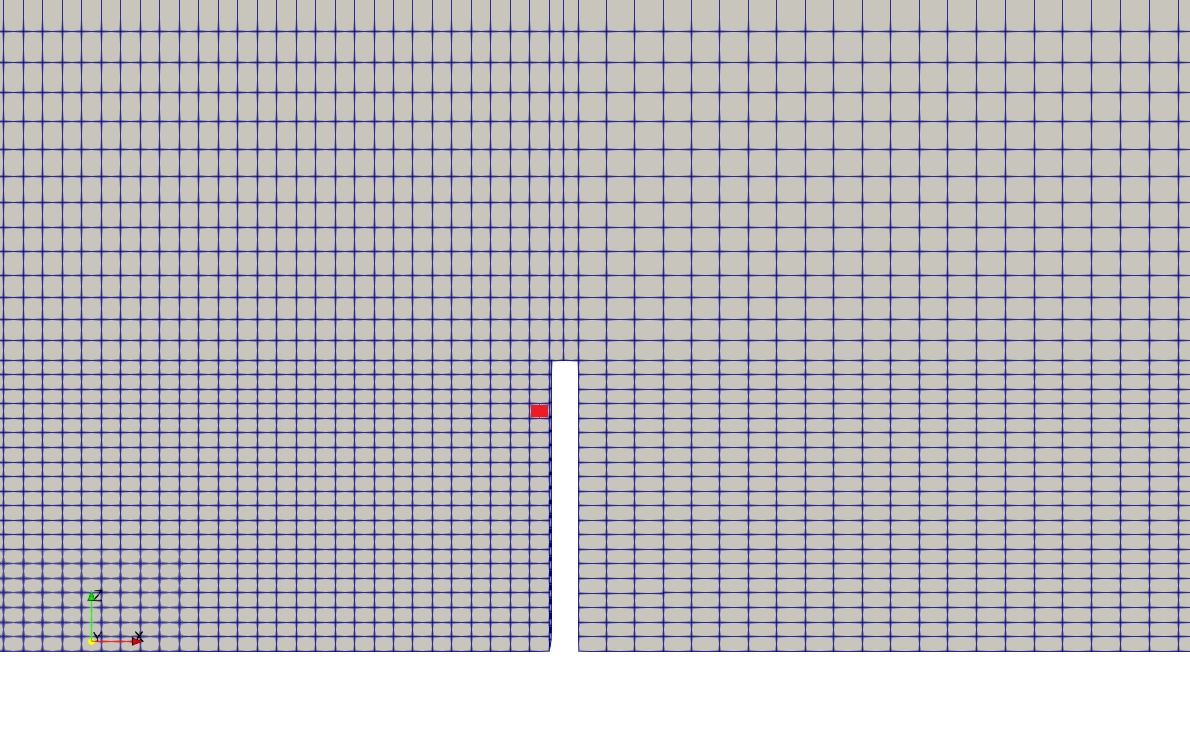
\includegraphics[width=.99\linewidth]{images/undist}
		\caption{undistorted mesh}
		\label{fig:undist}
	\end{subfigure}%
	\begin{subfigure}{.5\textwidth}
		\centering
		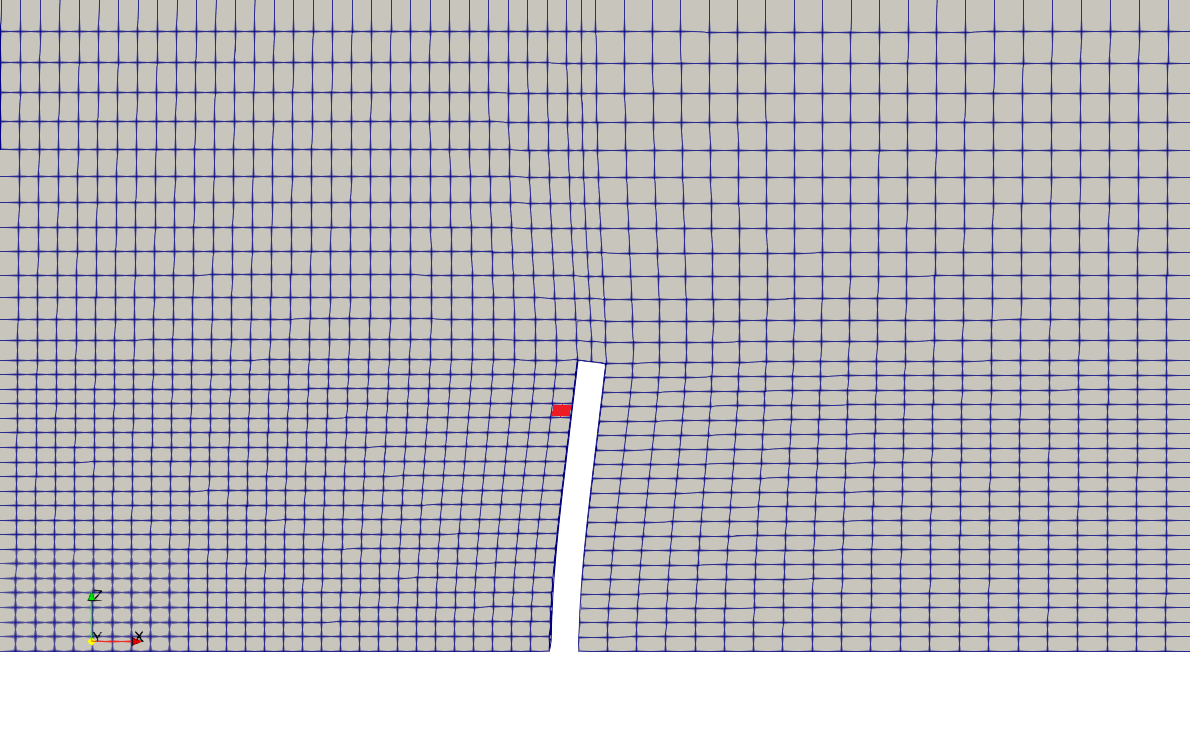
\includegraphics[width=.99\linewidth]{images/dist}
		\caption{distorted mesh}
		\label{fig:dist}
	\end{subfigure}
	\caption{ALE mesh}
	\label{fig:ale-mesh}
\end{figure}

\section{Domains and interface}
\label{sec:models}

Fluid-structure interaction implies that the overall model is determined by models defining the fluid behavior and the solid behavior, briefly described in sections \ref{sec:solid} and \ref{sec:fluid}. A short overview of beam models is given in section \ref{sec:beam} as it is relevant for the model developed in this work.
Finally a formal definition of the interface is given in section \ref{sec:interface}, as it is necessary to define suitable coupling conditions at the common boundary of the solid and the fluid.


\subsection{Fluid domain}
\label{sec:fluid}

An exhaustive description of all possible fluid models is far beyond the scope of this work. A quite general model is the viscous compressible one described by the ~\ac{NSE}. 

\begin{subequations}
\begin{eqnarray}
	\label{eq:cont}
	\frac{\partial{\rho}}{\partial{t}} + \nabla \cdot \left(\rho \vec{v}\right) &=&  0 \\	
	\label{eq:mom-cons} 
	\frac{\partial }{\partial t}\left( \rho \vec{v} \right) + \nabla \cdot \left( \rho \vec{v} \otimes \vec{v} \right) +\nabla p - \nabla \cdot \mathbf{\tau} - \rho \vec{g} &=& 0 \\
	\label{eq:energy-cons}
	\frac{\partial }{\partial t}\left( \rho e_0  \right) + \nabla \cdot \left( \rho e_0 \vec{v} \right) + \nabla \cdot \left( \vec{v}p + \vec{q} -\vec{v} \cdot \bm{\tau} \right) - \vec{v} \cdot \rho \vec{g} &=& 0
\end{eqnarray}
\end{subequations}

where:
\begin{itemize}
	\item $\rho$ denotes density
	\item $\vec{v}$ is flow velocity in all dimensions
	\item \textit{p} denotes pressure
	\item $\bm{\tau}$ is the viscous stress tensor
	\item $\vec{g}$ represents the sum of all body forces
	\item $e_0$ is the total energy per unit mass
	\item $\vec{q}$ is the heat flux by conduction
\end{itemize}

They consist in the mass conservation equation (\ref{eq:cont}), the conservation of momentum equation (\ref{eq:mom-cons}) and the energy conservation equation (\ref{eq:energy-cons}). For a Newtonian fluid, the viscous stress tensor is given by:

\begin{equation}
	\label{eq:tau}
	\bm{\tau} = -\frac{2}{3}\mu \left( \nabla \cdot \vec{v} \right) I +2\mu S
\end{equation}

with $\mu$ being the dynamic viscosity and \textit{S} the rate of deformation tensor (i.e. the symmetric part of the velocity gradient $\nabla \vec{v}$):

\begin{equation}
	\label{eq:def_tens}
	\mathbf{S} = \frac{1}{2} \left( \nabla \vec{v} + \nabla \vec{v}^T \right)
\end{equation}

A detailed derivation of such equations and the theory beyond can be found for example in  \cite{quartapelle2013fluidodinamicaI} and \cite{quartapelle2013fluidodinamicaC} or in \cite{pope2001turbulent}. 

The set of equations above, even with a Newtonian fluid model, lack some other information in order to form a closed set of ~\ac{PDE}. A conductive heat flux model is needed  (e.g. Fourier’s Law), the caloric and thermodynamic equations of state have to be chosen, a proper turbulence model if needed (see \cite{pope2001turbulent}) and finally, the appropriate initial and boundary conditions for the problem \cite{galdi2011introduction} must be defined.

Simplifications can be done to obtain less sophisticated models such as: adiabatic, inviscid, incompressible, and many others. Dimensional Analysis is a powerful tool to determine to what extent some reduced models are meaningful, and it is widely used in fluid dynamics, as described in section \ref{sec:dimensional}. Most CFD software codes allow to set up simulations with the most suitable model which can be coupled with a solid model to build a FSI problem. Some further details are given in section \ref{sec:monolithic}. 


\subsection{Solid domain}
\label{sec:solid}

In solid mechanics, particles do not travel as much as they do in fluid dynamic problems, as described in \ref{subsec:lagrange}. For this reason, a Lagrangian perspective is generally used.  

The  de-Saint Venant-Kirchhoff model \cite{ogden1997non} is very commonly used when describing the movement of a solid: it is also often used in FSI problems ad it is capable of handling large deformation. The material is considered:

\begin{itemize}
	\item \textit{homogeneous}: the material properties do not depend on the position of the particle
	\item \textit{linear elastic}: the stress-strain relationship is linear
	\item \textit{isotropic}: the stress-strain relationship is independent from the direction of the load
\end{itemize}

A general expression of the dynamic equation can be derived from the ~\ac{VWP} applied to an arbitrary control volume: 

\begin{equation}
	\label{eq:mech}
	\frac{\partial^2 \vec{u} }{\partial t^2} = \nabla \cdot \mathbf{T} + \rho \vec{f}
\end{equation}

In equation \ref{eq:mech}:

\begin{itemize}
	\item $\rho$: is the material density
	\item $\vec{u}$: is the particle displacement
	\item $\mathbf{T}$: is the \textit{second Piola-Kirchhoff} stress tensor
	\item $\vec{f}$: is the sum of body forces
\end{itemize}


In order to close the dynamic equation, a constitutive law which must be considered to relate stress and strain:

\begin{equation}
	\mathbf{T} = \lambda \mathbf{I} \mathrm{tr}\left[ \bm{\varepsilon_G}  \right]  + 2\mu \bm{\varepsilon_G}
\end{equation}

where $\bm{\varepsilon_G}$ is the Green-Lagrange strain tensor:

\begin{equation}
	\bm{\varepsilon_G} = \frac{1}{2}\left( \mathbf{F}^T \mathbf{F}-\mathbf{I}  \right)
\end{equation}

and $\mathbf{F}$ is the deformation gradient. $\lambda$ and $\mu$ are material properties and are named Lamé constants. These relate to the Young modulus \textit{E} and the Poisson ratio $\nu$ which are more commonly used in practice. The relationship among the various parameters is the following:


\begin{eqnarray}
	E &=& \frac{\mu(3\lambda+2\mu)}{\lambda + \mu} \\
	\nu &=& \frac{\lambda}{2(\lambda + \mu)}
\end{eqnarray}

The set of parameters $\left(E, \nu\right)$ or $\left(\lambda, \mu \right)$, together with the density $\rho$ fully define the material, under the assumptions of linear elasticity, isotropy and homogeneity.

The set of PDEs is completed when suitable initial and boundary conditions are defined.

\subsection{Models with reduced dimensionality: beams}
\label{sec:beam}

The equations introduced in section \ref{sec:solid} may be a tough task to solve even of the case of isotropic hyperelasticity, when considering a 3-D domain. Even with today's computers and using finite elements techniques, it is not always feasible or convenient to treat a solid as a three-dimensional continuum. Body with particular geometric features can be seen as lower dimension bodies, with respect to the governing equations \cite{hjelmstad2007fundamentals}. Such bodies are called \textit{beams} (one dimension) , \textit{plates} or \textit{shells} (two dimensions).

The \textit{beam} model splits the description of the geometry into two subproblems:
\begin{enumerate}
	\item a beam is defined by its \textit{reference line} and the movement (displacement and rotation) of the solid is completely defined by it (see Figure \ref{fig:beam-model}),
	\item the beam \textit{cross section} is considered as a whole, its movement depends on the movement of the reference line, stresses are generalized into \textit{resultants} (axial, bending, shear, torsional) which represent the aggregate effect of all of the stresses acting on the cross section. The constitutive properties of the section (axial, shear, torsion and bending stiffness) allow to relate stresses and deformations (by means of VWP) and close the problem.
\end{enumerate}


\begin{figure}[htbp!]
	\centering
	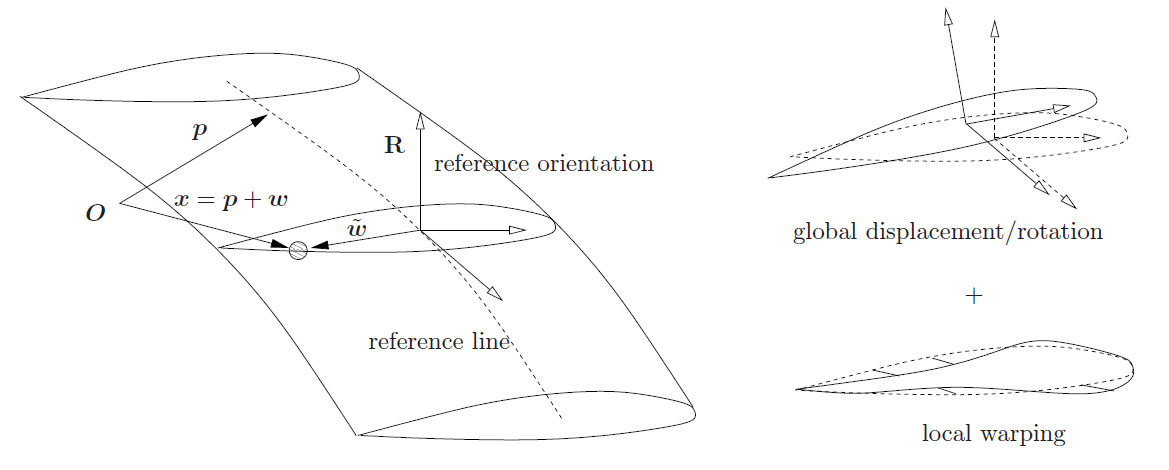
\includegraphics[width=0.8\textwidth]{images/beam}
	\caption{beam model, taken from \cite{ghiringhelli2008integrated}}
	\label{fig:beam-model}
\end{figure}


The beam model can be used to build elements of a ~\ac{FEM}. For example, the beam element can be modeled by means of a Finite Volume approach, as described in \cite{ghiringhelli2000multibody}, which computes the internal forces as functions of the straining of the reference line and orientation at selected points along the line itself, called evaluation points.

\hl{This approach is particularly interesting for FSI problems in which slender structures are involved. A mapping is needed between the fluid-solid interface and the reference line movement, which will be described in.}


\subsection{Interface and interaction}
\label{sec:interface}

Since FSI problems are centered on the interaction of the fluid and solid domain, their common interface needs to be described properly. A simple representation of the situation at the so called \textit{wet surface} is shown in Figure \ref{fig:interface}. Quantities related to the solid use S subscript, while fluid domain and the interface are labeled with F and FS, respectively. 

\begin{figure}[htbp!]
	\centering
	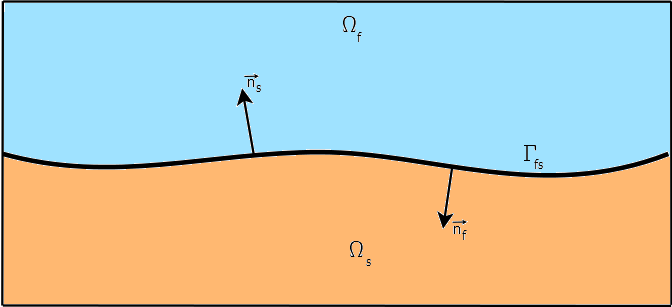
\includegraphics[width=0.8\textwidth]{images/interface}
	\caption{fluid solid interface}
	\label{fig:interface}
\end{figure}

In order to have a physically correct behavior, some conditions have to be met \cite{hou2012numerical}:

\begin{itemize}
	\item solid and fluid domains should not overlap nor separate,
	\item for a viscous fluid model, the flow velocity at the interface must equal the boundary velocity (\textit{no-slip} condition),
	\item for an inviscid fluid model, only velocity components normal to the wet surface have to be equal to the structural 	velocity as the fluid may slip freely in tangential direction at any boundary,
	\item forces exchanged at the interface must at equilibrium.
\end{itemize}

The first conditions result in the \textit{kinematical requirement} that the displacements of fluid and solid domains, as well as their respective velocities have to be equal at the wet surface (denoted by $\Gamma_{FS}$): 

\begin{eqnarray}
 \Delta\vec{x}_F &=& \vec{u}_S \\
 \vec{v}_F &=& \frac{\partial \vec{u}_S}{\partial t}
\end{eqnarray}

The last condition results in the equilibrium requirement. Force vectors are computed from the stresses at the interface and the outward normal vectors of fluid and solid domain, respectively. They have to be equal and opposite leading to the dynamic coupling condition:

\begin{equation}
\bm{\sigma_F} \cdot \vec{n}_F + \bm{\sigma_S} \cdot \vec{n}_F = 0
\end{equation}

$\bm{\sigma} \in \mathbb{R}^{3 \times 3}$ represents the stress tensor (note that for the fluid it comprises pressure and viscous stresses), while $\vec{n} \in \mathbb{R}$ is the outward normal unit vector.


\section{Classification of FSI problems}
\label{sec:classification}

In the previous chapters we have seen that there exist a lot of models that can describe fluid flow and solid mechanics. In FSI problems we need to couple two of them: the variety of coupled problems seems to be so large that  single FSI model that is applicable to every problem appears to be unfeasible. For this reason it is useful to classify FSI problems and look for specific properties in each class.  
The first step is to switch from dimensional quantities to dimensionless ones.


\subsection{Dimensional analysis}
\label{sec:dimensional}

We use the principle that a physical law should only relate to dimensionless quantities.  
There exist a rather general theorem called the $\Pi$ Theorem or the \textit{Vaschy-Buckingham Theorem} \cite{HancheOlsen2004}, which tells how many dimensionless quantities are needed to rewrite a model in dimensionless fashion.
This theorem states that the number of dimensionless quantities, P, is equal to that of the dimensional ones describing the problem, N, minus R, which is the rank of the matrix of dimension exponents. This matrix is formed by the columns of the dimension exponents of all variables \cite{hardtke2019buckingham}. An example is given in the following Section \ref{sec:dim-fluid}, Table \ref{table:dim-fluid}.

\subsection{Dimensional analysis in fluid domain}
\label{sec:dim-fluid}

Dimensional analysis is widely used in fluid dynamics. In order to keep the analysis simple,, we consider the adimensionalization of the incompressible Navier-Stokes momentum equation for a Newtonian fluid \cite{fox2020fox}:

\begin{equation}
	\frac{\partial \vec{v}}{\partial t} + \left(\vec{v} \cdot \nabla \right) \vec{v} = -\frac{\nabla p}{\rho} + \nu \nabla ^2 \vec{v} + \vec{g}
	\label{eq:inc-ns}
\end{equation}

The variables involved in equation \ref{eq:inc-ns} are the following:

\begin{itemize}
	\item \textit{t}: time
	\item $\vec{x}$: coordinates
	\item $\vec{v}$: velocity field
	\item \textit{p}: pressure field
	\item $\rho$: fluid density
	\item $\nu$: fluid kinematic viscosity
	\item $\vec{g}$: gravity
	\item \textit{L}: reference dimension
	\item $V_0$: reference velocity
\end{itemize}




\begin{table}[!h]
\begin{center}
	\begin{tabular}{ c|c c c c c c c c c} 
		  & \textit{t} & $\vec{x}$ & $\vec{v}$ & \textit{p} & $\rho$ & $\nu$ & $\vec{g}$ & \textit{L} & $V_0$  \\ 
		\hline
		L & 0 & 1 & 1  & -1 & -3 & 2  & 1  & 1 & 1  \\ 
		M & 0 & 0 & 0  &  1 &  1 & 0  & 0  & 0 & 0  \\
		T & 1 & 0 & -1 & -1 &  0 & -1 & -2 & 0 & -1 \\ 
	\end{tabular}
\end{center}
\caption{fluid  matrix of dimension exponents}
\label{table:dim-fluid}
\end{table}

The rank of the above matrix is 3 so 6 dimensionless parameters are needed to rewrite the equation \ref{eq:inc-ns}:

\begin{itemize}
	\item \textit{length}: $\vec{x}^* = \frac{\vec{x}}{L}$
	\item \textit{velocity}: $\vec{v}^* = \frac{\vec{v}}{V_0}$
	\item \textit{time}: $t^* = \frac{V_0 t}{L} = \frac{t}{T_{fluid}}$
	\item \textit{pressure}: possible choices: $p^* = \frac{p}{\rho V_0^2}$ or, if viscous forces are dominant, $p*= \frac{p L}{\rho \nu V_0}$
	\item \textit{Reynolds number}: $Re=\frac{V_0 L}{\nu}$. It defines the ratio between inertia and viscous forces.
	\item \textit{Froude number}: $Fr = \frac{V_0}{\sqrt{g L}}$. It defines the ratio between the flow inertia to the body field forces
\end{itemize} 


The adimensionalized momentum equation becomes:

\begin{equation}
	\frac{\partial \vec{v}^*}{\partial t^*} + \left( \vec{v}^* \cdot \nabla \right) \vec{v}^* = -\nabla p^* +\frac{1}{Re} \nabla^2 \vec{v}^2 + \frac{1}{Fr^2}\vec{g}
	\label{eq:adim-ns}
\end{equation}

From Equation \ref{eq:adim-ns} a lot of models might be derived: from \textit{Stokes regime} when viscosity is dominant, to \textit{Euler regime} when viscosity is negligible with respect to inertia forces.


\subsection{Dimensional analysis in solid domain}

Even if it is seldom used, Dimensional Analysis can be made also for the solid domain \cite{longo2011analisi}.

The variables involved in a solid dynamics equation are:

\begin{itemize}
	\item \textit{t}: time
	\item $\vec{X}$: coordinates
	\item $\vec{u}$: displacement field
	\item $\rho_S$: solid density
	\item \textit{E}: elastic modulus
	\item $\vec{g}$: gravity
	\item \textit{L}: reference dimension
	\item $U_0$: reference displacement
\end{itemize}

From the variables above the following parameters can be derived:

\begin{itemize}
	\item \textit{length}: $\frac{\vec{X}}{L}$: dimensionless coordinate
	\item \textit{displacement}: $\frac{\vec{u}}{L}$: dimensionless displacement
	\item \textit{time}: $\frac{t \sqrt{\frac{E}{\rho_S}}}{L} = \frac{t}{T_{solid}}$ dimensionless time
	\item entity of displacements: $\frac{U_0}{L} = \delta$: \textit{displacement number}
	\item gravity: $\frac{\rho_S g L}{E}$: elastogravity number
\end{itemize}

$T_{solid}$ can be seen as $\frac{L}{c}$ with $c = \sqrt{\frac{E}{\rho_S}}$ which is the scale of elastic wave velocity. The displacement number $\delta$ tells how big the structure displacement are related to the overall dimension, and defines the \textit{large displacements} region.
Finally, the \textit{elastogravity number} combines gravity (or body forces in general), density and stiffness: when large the deformation induced by body forces in the solid are large. 

\subsection{Dimensional analysis of coupled problems}

It is now possible to undertake the dimensional analysis of a fully coupled fluid and solid interaction problem. Some of the parameters are only defined in the fluid side or in the solid side (e.g. viscosity or stiffnes). Some parameters are common to both domains (e.g. lenght scale or gravity). The variables of interest are now the velocity in the fluid and the displacements in the solid. Each of them can be related to all the parameters without separation. For example, the fluid velocity relationship is of the kind:

\begin{eqnarray}
	 g(\vec{v}; \vec{x},t; \rho, \mu, V_0; \rho_S. E; \vec{g}, L) = 0
	 \label{eq:vel-param}
\end{eqnarray}


Equation \ref{eq:vel-param} is composed of 11 dimensional parameters. Applying $\pi$ theorem, the total number of independent dimensionless parameter expected is 8. Starting from the ones derived in the previous sections:

\begin{itemize}
	\item $\vec{x}^* = \frac{\vec{x}}{L}$: dimensionless coordinates
	\item $\vec{v}^* = \frac{\vec{v}}{V_0}$: dimensionless fluid velocity
	\item $t*_f = \frac{V_0 t}{L}$: dimensionless time
	\item $Re = \frac{V_0 L}{\nu}$: Reynolds number
	\item $Fr = \frac{V_0}{\sqrt{gL}}$: Froude number
	\item $\delta = \frac{U_0}{L}$: displacement number
	\item $\frac{\rho_S g L}{E}$: elastogravity number
\end{itemize}

The 7 quantities above derive from the separated problem. The last one necessarily mixes things from the fluid and the solid side otherwise it would have been found in one uncoupled case. There is no unique choice for this parameter, the following are the most common ones.

\subsubsection{Mass number}

The simplest, but arguably most important parameter is the ratio of the two densities: the \textit{Mass Number} M.

\begin{equation}
	M = \frac{\rho}{\rho_S}
	\label{eq:mass-number}
\end{equation}

This can range from $\mathcal{O}\left(10^{-4}\right)$ in air-steel interaction to $\mathcal{O}\left(1\right)$ when both media have about the same density. This parameter is particularly significant for the so called \textit{added mass} stability problem, described in Section \ref{sec:added-mass}.

\subsubsection{Reduced velocity}

Another possible choice is the reduced velocity:

\begin{equation}
	 U_R = \frac{V_0}{\sqrt{\frac{E}{\rho_S}}}
\end{equation}

It is the ratio between the fluid free velocity and the velocity of elastic waves in a solid, \textit{c}. It contains information on the way the two dynamics are related and it can range different orders of magnitude.

\subsubsection{Cauchy number}

Another possible parameter combines stresses or stiffness: the  Cauchy number, as defined in \cite{de2001fluides}:

\begin{equation}
	C_Y = \frac{\rho V_0^2}{E}
\end{equation}

It is the ratio between the fluid inertial forces, quantified by the dynamic pressure and the stiffness of the solid E. 
The higher it is, the more the solid is elastically deformed by the flow.


These are actually the most important parameters involving FSI problems. Among them, there is no universally better choice. But there are efficient choices, that would be more helpful
in solving a given problem. 


